\begin{figure}[H]
  \centering
  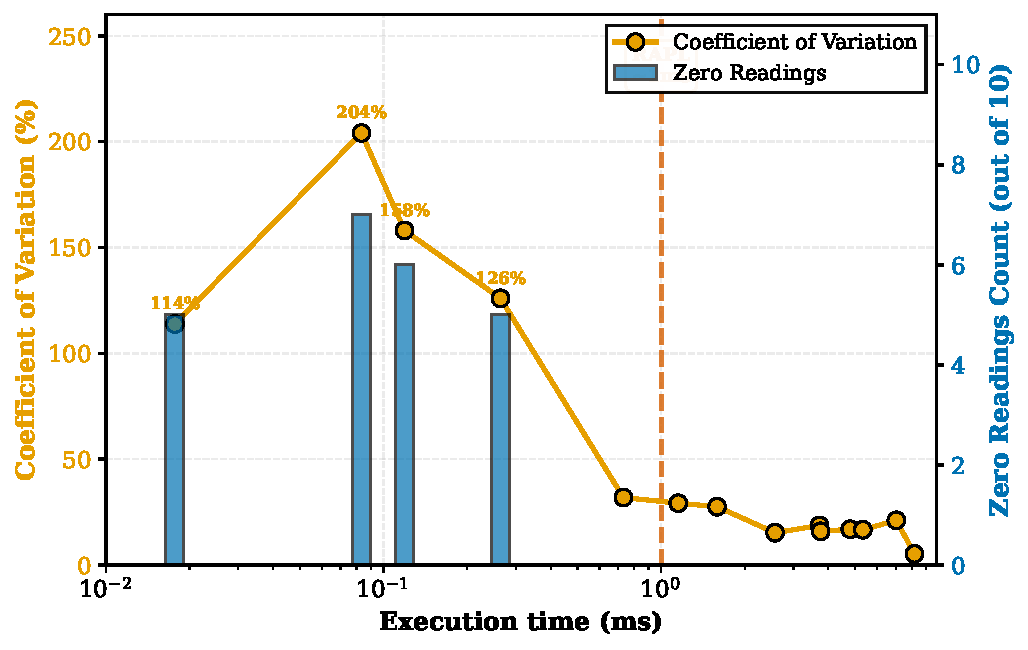
\includegraphics[width=\linewidth]{figures/rapl_paper_quality.pdf} 
  \caption{Quality of RAPL's Measurements over Execution Time of the Workload (ms in Log scale)}
  \label{fig:rapl-quality}
\end{figure}
\section{Motivation}
\label{sec:motivation}
% 1. The Core Challenge in detail 
% A Motivation Example

Developing energy efficient software would require reliable insight into how individual fragments of source code contribute to energy consumption. Existing measurement techniques use hardware based counters such as Intel's Running Average Power Limit (RAPL). While effective for coarse grained profiling, but RAPL's millisecond resolution is too large for such code fragments. As Figure~\ref{fig:rapl-quality} demonstrates that workloads under 1ms register more than 110\% variation and 4-5 runs get zero readings (out of 10 runs). Even above 1ms, the variation is significant. Although hardware power meters provide higher resolution, they are severely limited in terms of accessibility, reproducibility, and usability in distributed systems. To address this fundamental limitation, we developed \textbf{PowerLens}, a methodology for obtaining precise and reproducible energy readings at sub-millisecond granularity. However, accurate measurements alone are insufficient; developers need energy information before code execution. To enable this, we propose \textbf{EnCoDe}, which trains machine learning models on PowerLens measurements to predict block-level energy consumption directly from source code features, shifting energy assessment from a runtime profiling concern to a proactive design-time estimation.

 % \cite{ALVI2021100594} \cite{inproceedings} \cite{10.1145/2425248.2425252}

\begin{comment}

\begin{figure*}[htbp]
  \centering
  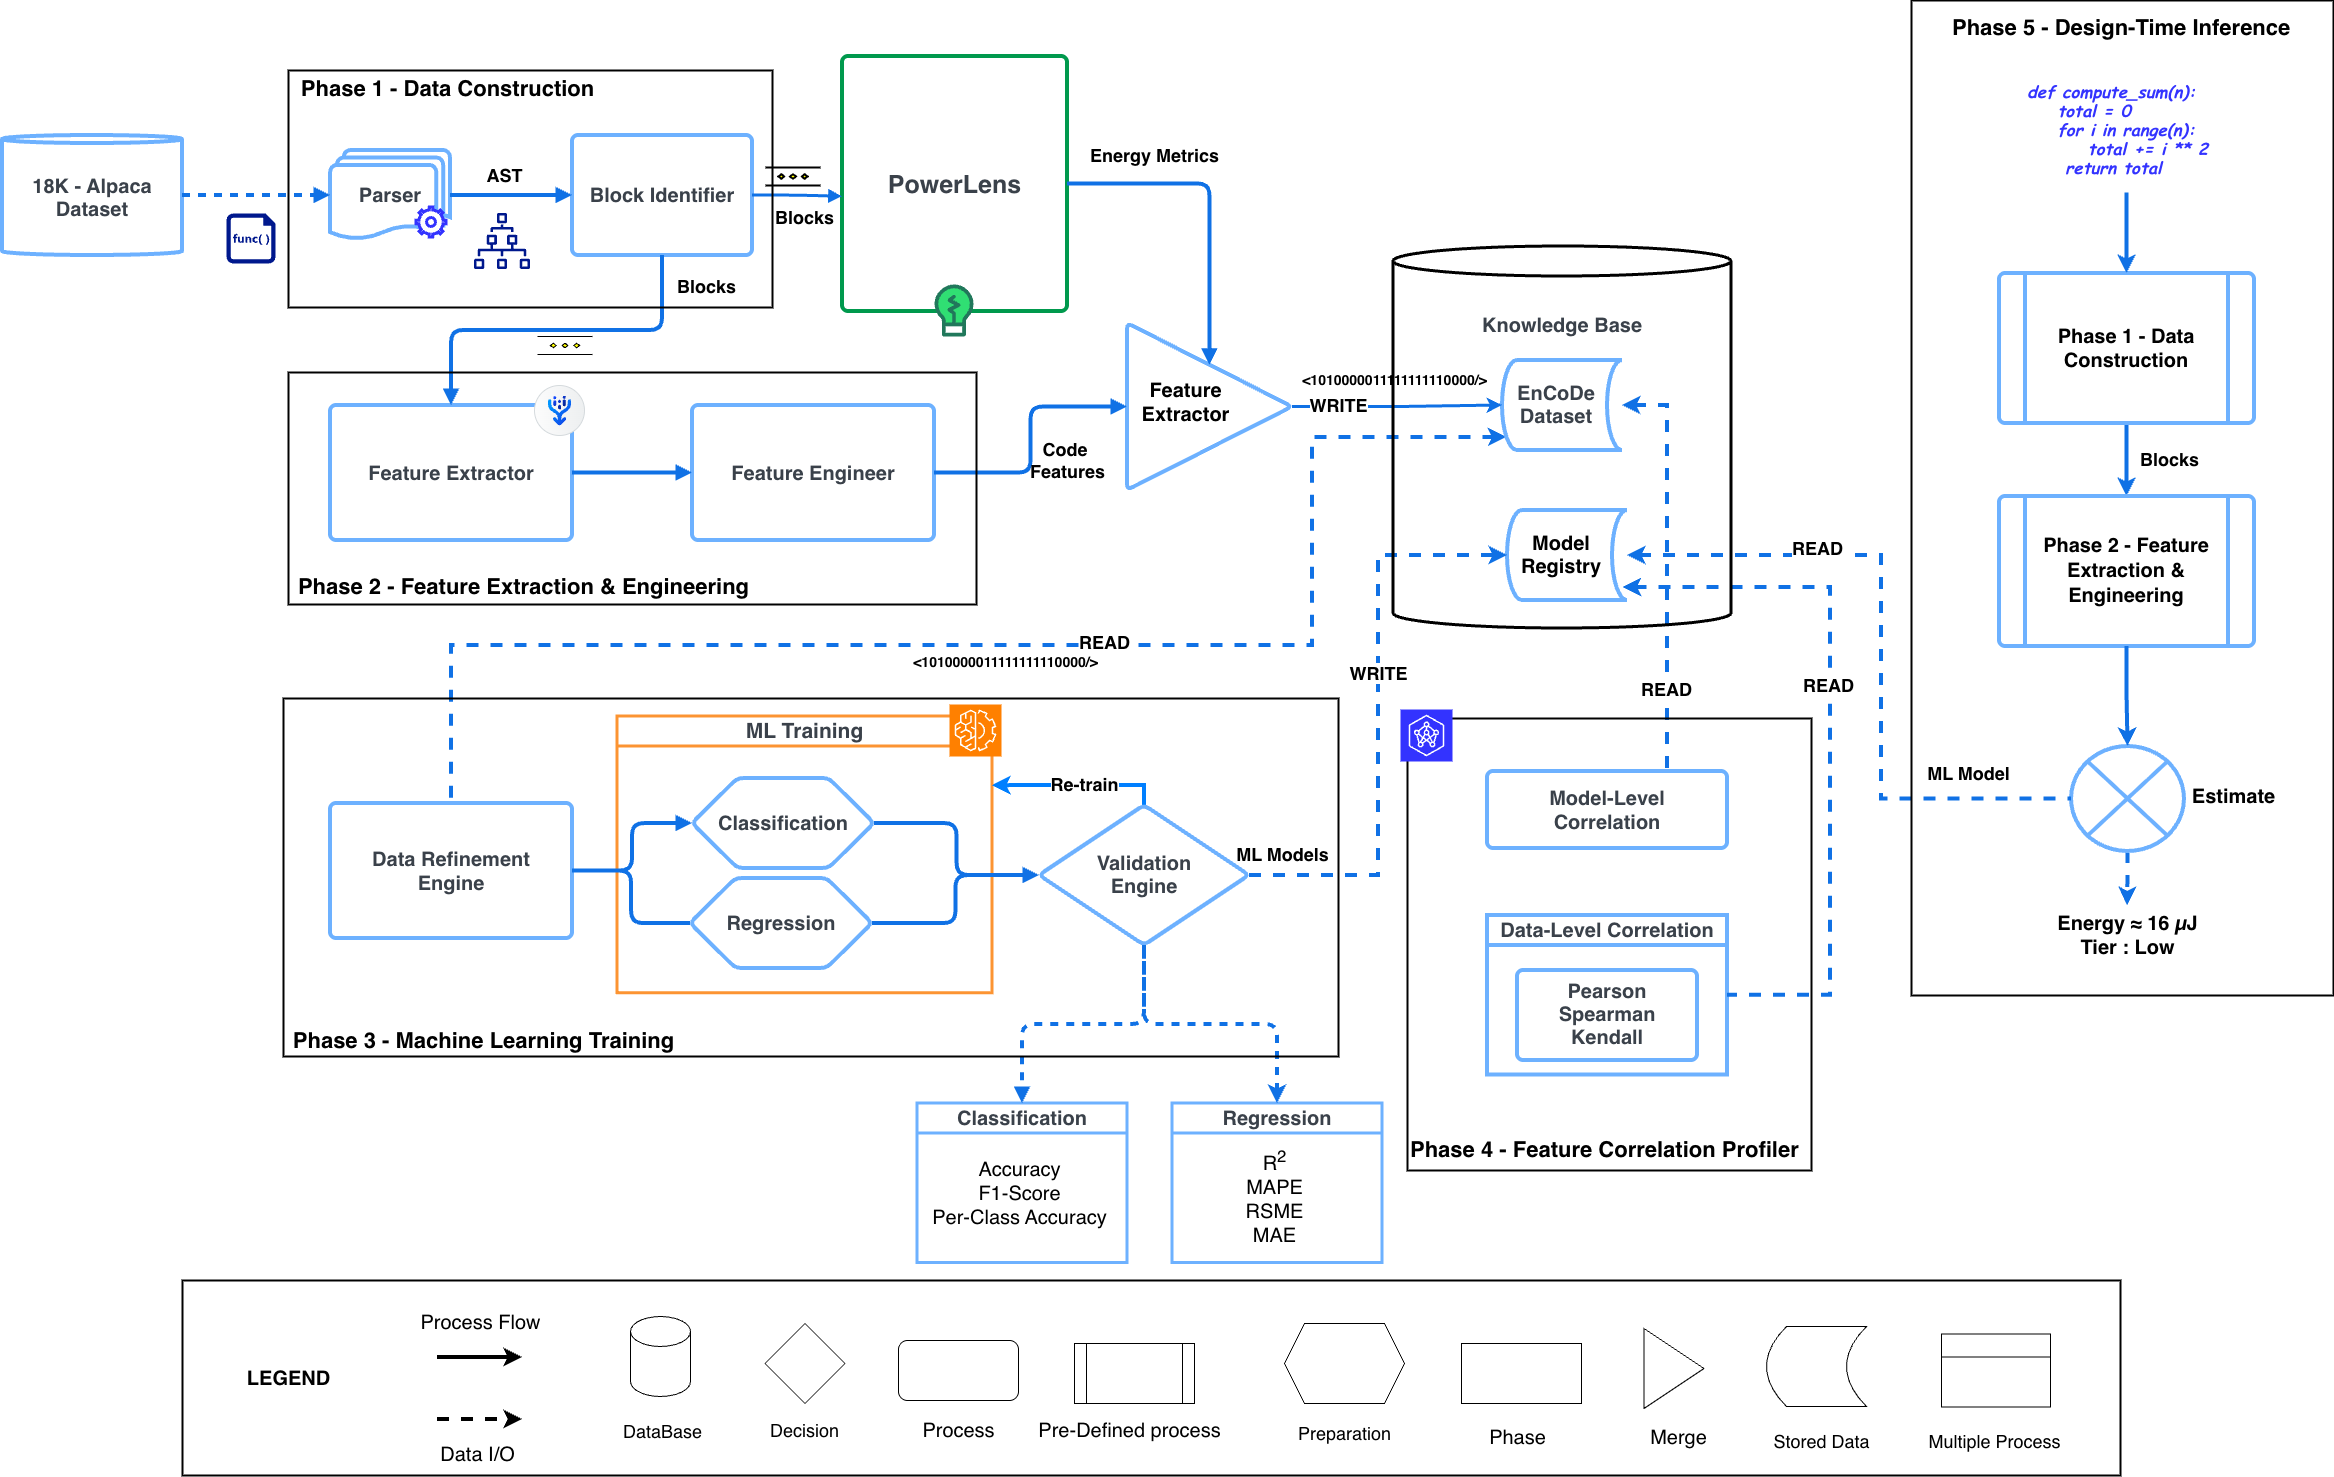
\includegraphics[width=0.95\textwidth]{figures/EnCoDe.png}
  \caption{Design Time Energy Estimation Framework}
  \label{fig:framework}
\end{figure*}

\end{comment}